\subsection{GraphGPS with HIG}
GraphGPS is by design a highly malleable model, which allows for easy additions to the code. Thus we implemented HiG in a section of GraphGPS.

\begin{figure}[ht]
    \centering
    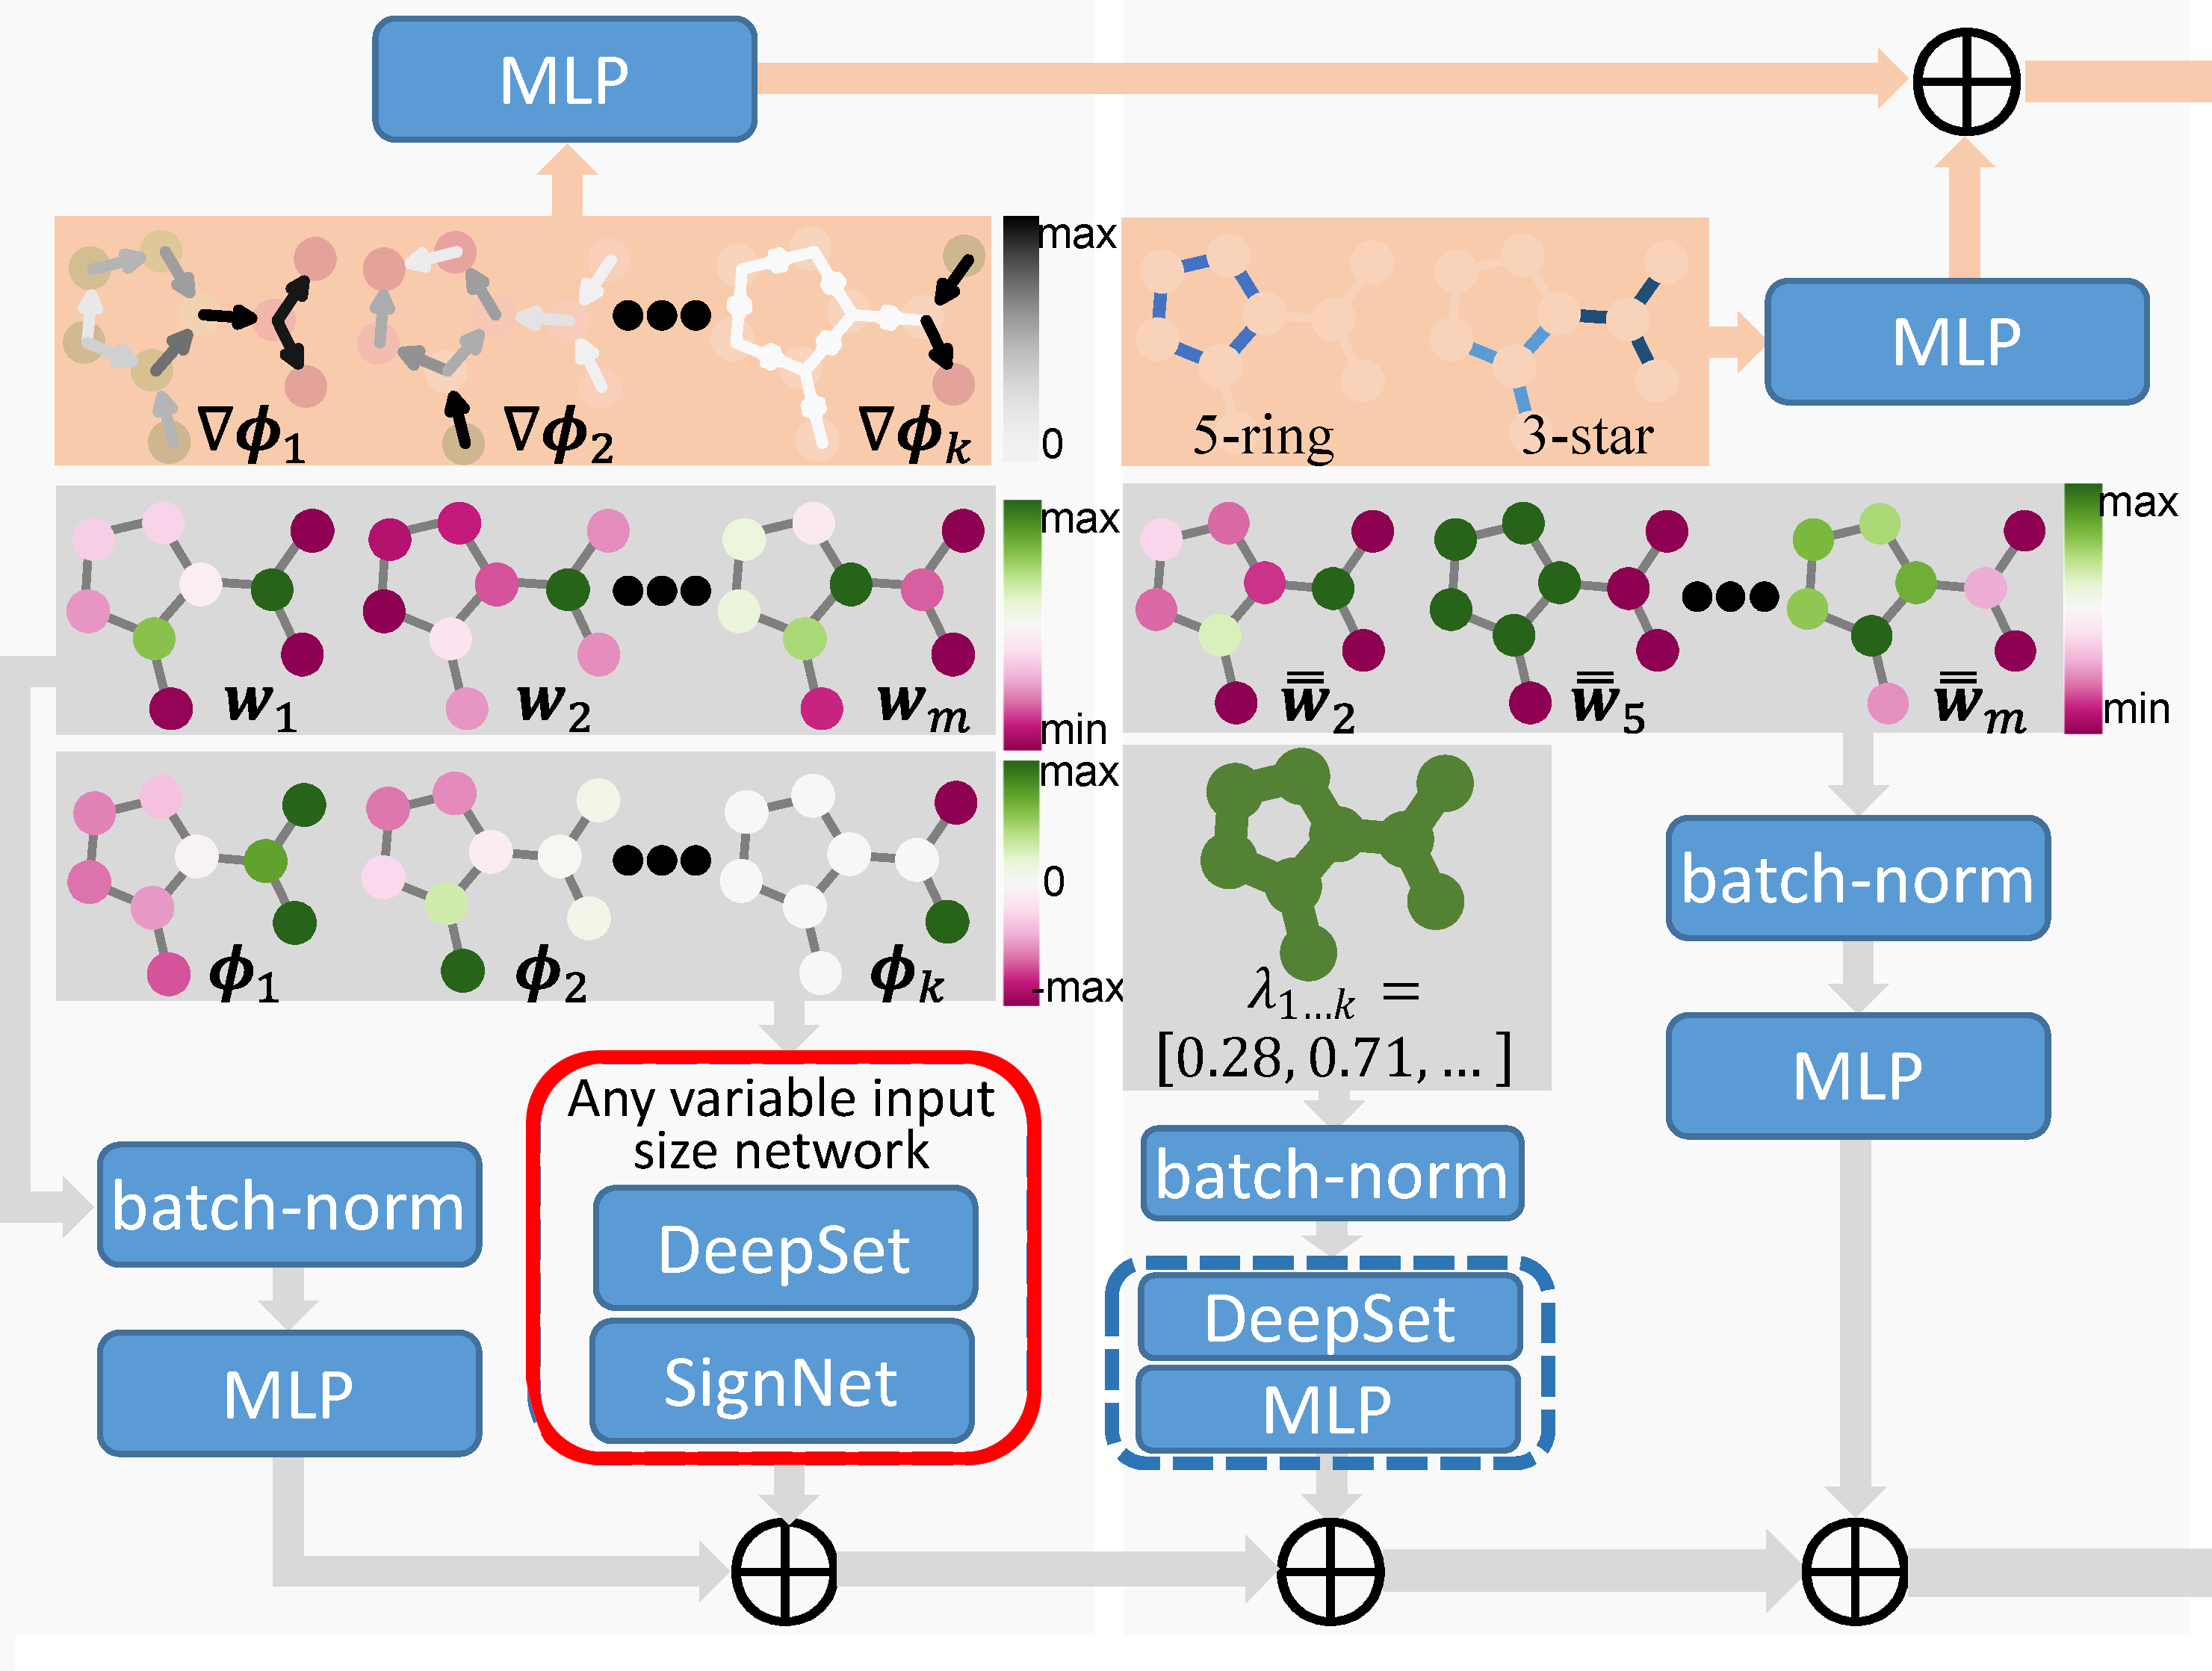
\includegraphics[scale=0.2]{tex/res/gps_hig_position.png}
    \caption{Position of our approach in the architecture}
    \label{fig:gps-hig-position}
\end{figure}

\subsubsection{Implementation}

\begin{lstlisting}[style=cpp,caption={HiG-Code in GraphGPS},label={lst:Void},numbers=left]
if 'HIG' in pe_types:
    interpolation_chance = cfg.posenc_HIG.loss
    is_interpolating = np.random.choice(2, 1, p=[1-interpolation_chance,interpolation_chance])[0]
    minimum_node_size = cfg.posenc_HIG.minimum_node_size
    nodes_interpolated = cfg.posenc_HIG.nodes_interpolated
    minimum_node_size = max(minimum_node_size, nodes_interpolated)
    if data.num_nodes > minimum_node_size and is_interpolating == 1:
        rand_ints = np.random.choice(data.num_nodes, nodes_interpolated, 
	    replace=False)
        sum = {}
        for rand_int in rand_ints:
            data.x[rand_int] = 0
            sum[rand_int] = 0
        for i in data.edge_index[0]:
            if i in rand_ints:
                relevant_node = data.edge_index[1][i]
                data.x[i] = torch.add(data.x[i], data.x[relevant_node])
                sum[i] += 1
        for rand_int in rand_ints:
            data.x[rand_int] = data.x[rand_int] / sum[rand_int]
\end{lstlisting}

\subsubsection{Results}

\begin{table}[ht!]
    \centering
    \caption{Node feature vector}
    \label{node_features}
    \begin{tabular}{c || l| p{6cm} |}
        Feature            & Feature-Specialization & Test-AUC \\
        \hline
        \hline
        Normal HiG         &                        & 0.75274  \\
        \hline
        Loss               & 0.5                    & 0.77894  \\
                           & 0.1                    & 0.77033  \\
                           & 0.01                   &          \\
        \hline
        Nodes Interpolated & 2                      & 0.73967  \\
                           & 3                      & 0.73882  \\
                           & 5                      & 0.71498  \\
        \hline
        min. graph size    & 5 nodes                &          \\
                           & 10 nodes               & 0.76795  \\
                           & 20 nodes               & 0.77084  \\
                           & 50 nodes               & 0.7566   \\
    \end{tabular}
\end{table}
